%
%                       This is a basic LeTeX Template
%                       for the First Year Summary 
\documentclass[a4paper,12pt]{article}
\usepackage{head,fullpage}    % Add local fullpage macros
\usepackage[pdftex]{graphicx} % Graphicx package with pdf support
\usepackage{subcaption}
\usepackage{tabularx}
\parindent=0pt          %  Switch off indent of paragraphs 
\parskip=5pt            %  Put 5pt between each paragraph 
\footruleheight{1pt}
\headruleheight{1pt}
\lfoot{\small School of Physics and Astronomy}
\lhead{First Year Summary}
\rhead{- \thepage}
\cfoot{}
\rfoot{Date: 23-5-18} 
%
%                       This section generates a title page
%                       Edit only the sections indicated to put
%                       in the project title, your name, supervisor,
%                       project length in weeks and submission date
%
\begin{document}
\begin{minipage}[b]{110mm}
        {\Huge\bf School of Physics \\and Astronomy
        \vspace*{17mm}}
\end{minipage}
\hfill
\begin{minipage}[t]{40mm}               
        \makebox[40mm]{
        
\includegraphics[width=40mm]{crest}}
\end{minipage}
\par\noindent                                           % Centre Title, and name
\vspace*{5mm}
\begin{center}
        \Large\bf Modelling the growth of microbial populations in heterogeneous antimicrobial concentrations\\
      
        \Large\bf First Year Summary
\end{center}
\vspace*{3mm}
\begin{center}
        \bf Patrick Sinclair\\                 % Replace with your name
        May 2018                         % Submission Date
\end{center}
\vspace*{5mm}
{\bf Supervisor:} Dr. Rosalind Allen                % Change to suit

%                                               Through page and setup 
\section{Project Outline}

Antimicrobial resistance is one of, if not the, most important issue in modern medicine.  Despite the massive prevalence of antibiotic usage, with over 260,000,000 prescriptions 
being issued in the US alone each year, surprisingly little is known about the underlying pharmacodynamics, and what factors influence the emergence of resistance.  This lack 
of understanding is becoming increasingly critical as our supply of viable antibiotics dwindles in comparison to the increasing number of resistant strains of bacteria.  In 
2014 there were over 480,000 cases of drug-resistant tuberculosis reported, with only half of those cases able to be successfully treated.  Experts estimate that if current trends 
continue, the number of deaths caused by drug-resistant bacteria will number in the millions, making further research in the field vital.

Statistical physics perspectives can play an important role in understanding the emergence of resistance.  This project therefore aims to 
use stochastic computational modelling techniques to glean insight on how the presence of antimicrobials control microbial colonies that form on surfaces from a more physics based 
perspective.  In particular, this project aims to investigate the underlying dynamics which influences how microbial populations, e.g. biofilms, form and proliferate when exposed 
to spatially heterogeneous drug concentrations.

While copious research has been undertaken on the mechanisms of how antibiotics kill or inhibit the growth of bacteria, the majority of these have been performed under very idealised 
conditions; with uniform antibiotic and nutrient concentration, and monospecies populations.  However, recent developments suggest that real-world factors which are neglected 
in these scenarios, play an important role over the development of these microbial populations.  In particular, how drug gradients allow microbes to expand spatially, 
the effects of differing nutrient-dependent growth rates on antimicrobial susceptibility, and competition between species with differing physiological attributes.

This project aims to utilise stochastic modelling techniques to investigate how these parameters affect the growth and development of microbial populations, and their expansion 
along antimicrobial gradients.  While these findings will obviously have important medical applications, they could also be of benefit in more industrial applications.  In particular, 
impeding, or even halting the formation of biofilm formation on industrial shipping vessels.  The shipping industry currently consumes an exorbitant amount of fuel.  
If it was a sovereign nation, it would be the 7$^{\textrm{th}}$ largest producer of CO$_2$ on the planet and it's estimated that up to 45\% of this fuel consumption in some cases 
is spent overcoming the additional drag caused by the formation of marine biofilms.  Therefore any progress in our ability to reduce the impact of this biofouling would be of 
great economic and environmental significance.  

Meetings with our industrial partner AkzoNobel has promoted discussions into the effects, and optimal design for antimicrobial paints.  These coatings are currently the industry 
standard for controlling marine biofouling, so research into how factors such as combinations of anti-microbials, and the release rates thereof affect biofilm development is key.  

The clinical and industrial aspects of my project have an interesting symmetry with each other.  In clinical situations, antibiotics are applied to the external surface of the 
biofilm, but in the industrial scenario the antimicrobial paints leach antimicrobials from the same surface as the biofilm is attached to.  Considering these two scenarios will allow 
me to investigate whether the direction of the gradient also has a role in how microbial populations proliferate through space.

\subsection*{Progress so far}

So far I have performed several investigations into the effects of antimicrobial gradients on the evolution and proliferation of bacterial colonies.  The first project 
undertaken was to replicate the results of a PRL paper co-authored by my supervisor, which modelled how the steepness of antibiotic gradients in conjunction with differing 
mutational pathways affected the time taken for resistance to emerge.  This was primarily intended as a ``warm-up'' project, in order to gain familiarity with modelling these 
sorts of systems, and to build a foundation upon which further projects could be built. These simulations consisted of a simple 1D system comprising several interconnected 
microhabitats each of which had a carrying capacity and concentration of antibiotic, which both affected the growth rate of the bacteria within.  

Once I had set up this system, I began work on my first PhD research project.  Here, research was performed on the differing effects of growth-rate dependent antibiotics, and their 
comparative abilities on impeding the spatial expansion of an initial inoculation of bacteria.  Two systems were constructed, one with antibiotics which were more effective 
against fast-growing 
bacteria, the other with slow-growing bacteria targeting antibiotics.  In this model, the carrying capacity factor was replaced with a parameter which represented the concentration 
of nutrients remaining in the microhabitat, each replication which occurred resulted in nutrients being consumed.  This corresponded to a reduction in the overall growth rate,
which in turn altered the susceptibility of the bacteria to the applied antibiotic.  

\begin{figure}[h!]
 \centering
 \begin{subfigure}[h]{0.45\textwidth}
 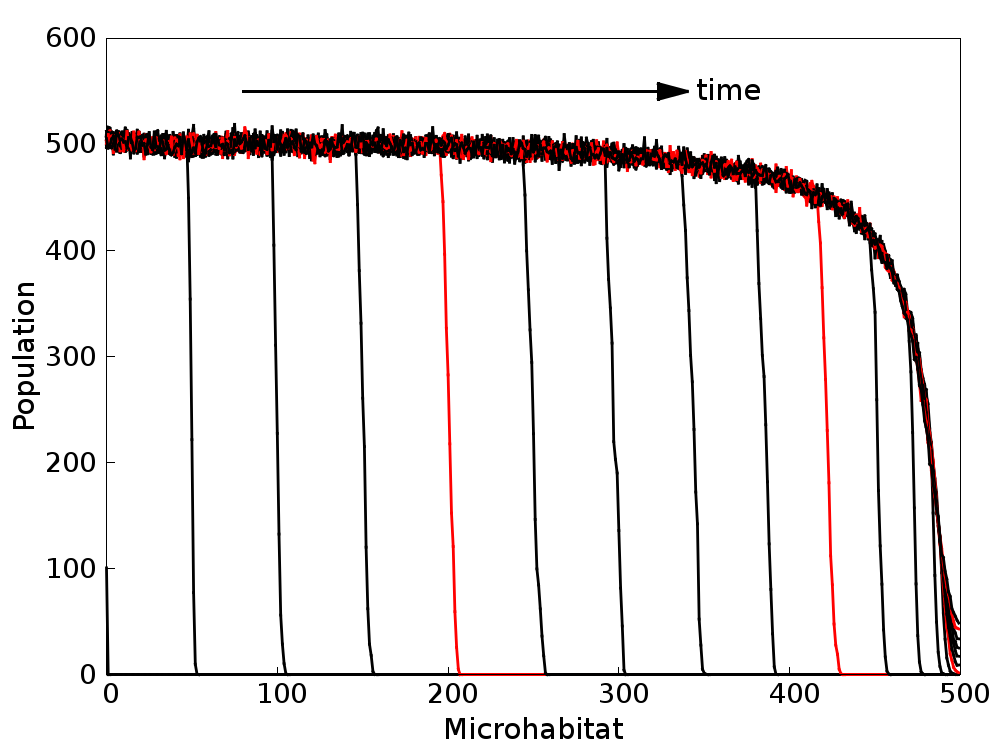
\includegraphics[width=\textwidth]{simple-slowGrowers-alpha=0_004884694070738408-spatialDistb}
  \caption{SGBTA}
  \label{subfig:SGBTA-spatdistb-spef_alpha}
  \end{subfigure}
  \begin{subfigure}[h]{0.45\textwidth}
  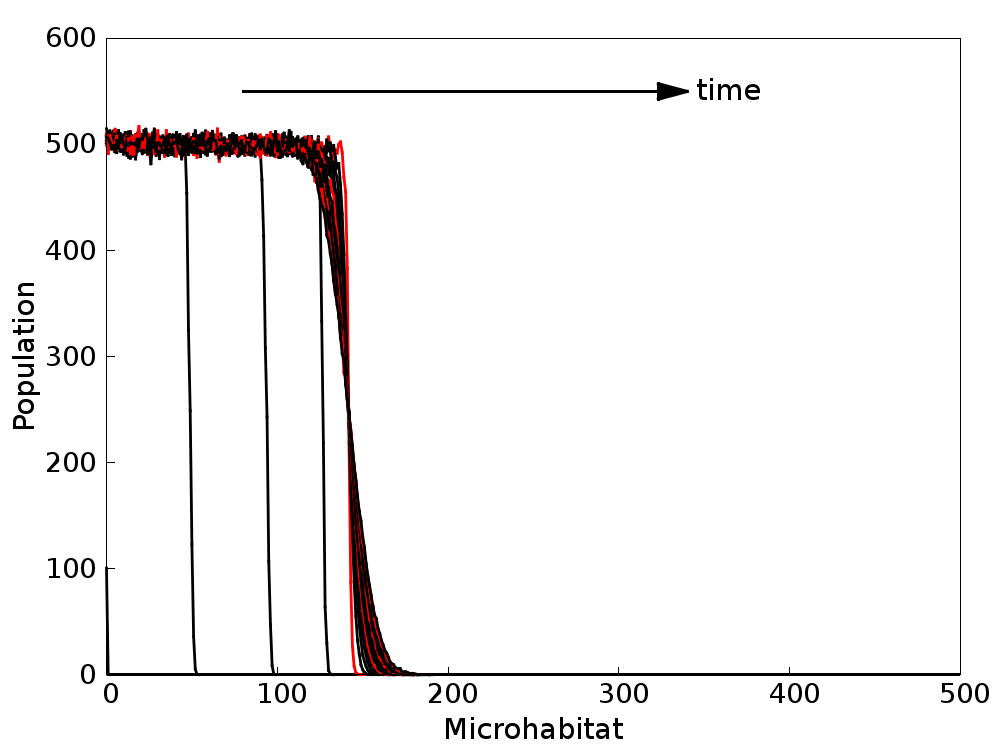
\includegraphics[width=\textwidth]{simple-fastGrowers-alpha=0_004884694070738408-spatialDistb}
  \caption{FGBTA}
  \label{subfig:FGBTA-spatdistb-spef_alpha}
 \end{subfigure}
\caption{Spatial distributions of bacterial populations exposed to SGBTA and FGBTA respectively, sampled over regular intervals.  The steepness of the antibiotic gradient has been 
chosen here such that the concentration does not reach the MIC until the last few microhabitats.  As can be seen, the SGBTA is inferior at inhibiting bacterial growth.}
\label{fig:alpha-spatdistbs}
\end{figure}

By sampling the spatial distribution of the bacteria over regular intervals, a comparison could be drawn to the differing efficacies of the two sets of antibiotics in curtailing 
population expansion.  As can be seen in Figure \ref{fig:alpha-spatdistbs}, the antibiotic which targets the fast-growing tip of the advancing population is more effective at 
inhibiting the spatial expansion of the population than the drug which targets the slow growing bulk towards the rear of the colony.  These experiments were repeated for a variety of 
gradients, uniform concentrations and with more realistic growth curves taken from in vitro experiments performed in laboratory conditions.  The corresponding results have now been 
collated and are in the process of being written up into a paper intended for publication.

Work has also begun on a simple multispecies model.  This model is similar to the ones mentioned previously, but consists of several species of microbe, each of which have differing 
growth rates.  This project aims to investigate the effects of interspecies competition, and the trade-off between time taken for the most resistant species to become dominant and 
the resulting population size, as a function of the steepness of the antimicrobial gradient.

\subsection*{Outlook}

Following a meeting with our industrial partners AkzoNobel, it was decided that work would continue for the meanwhile on the nascent multispecies model.  They mentioned how 
designing the right combination and release schedule of antimicrobials in order to promote the emergence of favourable biofilm compositions was of particular interest to them, 
so they intend to send us data on various bacterial species and their corresponding growth rates/susceptibilities to several biocides such that they could be incorporated into 
the multispecies model in order to deliver more quantitative results.

For future projects, it's planned that we will move away from the discrete 1D microhabitat model and begin work on a more intricate continuum model.  This would allow for the 
incorporation of more realistic dynamics such as flow, surface roughness and diffusion of the antibiotics, rather than the current fixed gradients.

% Outline of your project, covering the scientific background, the rational
% for your intended area of study and {\bf your progress to date}. 
% This should concentrate on why this subject
% area is important, interesting, worth studying and where you hope/believe your
% work will lead. You should also describe the context of your PhD � how does it fit into the international agenda?
% 
% This section should be 2-3 pages and written for the {\em general scientific
% reader}, (the typical reader of New Scientist, and in particular
% should {\it not} include any mathematical derivations.)
% 
% The whole report {\em must not} exceed {\bf four} pages.

\section{Critical Dependencies}

As this is a predominantly computational project, there aren't a large number of critical dependencies to consider.   Computation time has yet to become too much of an issue, 
but as the complexity of the model increases, it may do.  Usage of clusters such as Eddie etc. shoul alleviate these concerns.  There are currently plans for lab work to be 
performed with AkzoNobel at their complex in Newcastle, so this will depend on the availability of their apparatus.  However this aspect is only intended to form an 
interesting aside, rather than a key component of the project, so it should not be too much of a concern.


  
\section{Training and Courses}


{\bf Courses Attended in First Year}
\begin{center}
\begin{tabular}{l|c|c|c}
  Name    &     Origin    & Assessed   & Hours\\
  \hline
  Intro to Soft Condensed Matter    &     SUPA      & Yes        & 20\\
  Physics of Biological Evolution & SUPA         & Yes         & 10\\
  Maths Primer & SUPA & Yes        & 6\\
  Python & SUPA & Yes & 8\\
  Preparing for the first year review & Transkills & No & 3
\end{tabular}
\end{center}



{\bf Courses to be Attended in 2018-2019}
\begin{center}
\begin{tabularx}{0.8\textwidth}{|X|c|c|}
  \hline
  Name    &     Origin    & Assessed \\
  \hline
  \hline
  Computational principles \newline to organize complexity & Summer school - INPHYNI & No\\
  \hline
  Advanced Data Analysis & SUPA & Yes\\
  \hline
  Introducing Biology to \newline Physicists & SUPA & Yes\\
  \hline
  Hands-on Writing & Transkills & No\\
  \hline
\end{tabularx}
\end{center}

\section{Teaching}
\begin{center}
\begin{tabular}{l|c|c}
  Name     &    Semester   & Hours\\
\hline
  MfP1 Tutorials & 1 & 40\\
  Practical Physics (SciProg) & 1 & 15 \\
  Physics 1B Labs & 2 & 30\\
\end{tabular}
\end{center}

I intend to undertake a similar amount of teaching in my second year, but most likely in different courses.
 

\end{document}

